\chapter{Estudo de Caso }
% : Requisitos, Organização, Métodos, Design, Implementação e Testes
\label{cap:estudo_caso}
Este capítulo apresenta o contexto, os requisitos, a organização, os métodos, o design, a implementação e os testes realizados no desenvolvimento do estudo de caso em uma plataforma de notícias sobre tecnologia chamada WallTech.

\section{Contexto}
\label{section:contexto}
O estudo de caso é realizado em uma empresa fictícia chamada WallTech, uma plataforma de notícias sobre tecnologia que tem como objetivo fornecer conteúdos atualizados e relevantes sobre inovações e tendências do setor. Nela, os usuários podem acessar e buscar notícias utilizando palavras-chave, tanto em dispositivos móveis quanto em computadores, graças ao design responsivo da aplicação.  

Visando melhorar a experiência do usuário (UX) e otimizar o desempenho da plataforma, os gestores de tecnologia da WallTech decidiram realizar um estudo comparativo entre duas abordagens de renderização: \acrfull{csr} e \acrfull{ssr}. Para isso, optou-se pelo desenvolvimento de dois protótipos da plataforma, um com \acrshort{csr} utilizando React e outro com \acrshort{ssr} utilizando Next.js, com o objetivo de analisar qual modelo de renderização apresenta melhores resultados em termos de velocidade de carregamento, interatividade e no \english{\acrfull{seo}}.

A Figura \ref{fig:caso-uso-walltech} apresenta o diagrama de caso de uso da plataforma WallTech, mostrando as principais funcionalidades disponíveis para o usuário anônimo. O diagrama ilustra as interações do usuário com o sistema, permitindo que ele visualize a lista de notícias mais recentes, acesse os detalhes de uma notícia ao clicar nela, ou realize buscas específicas utilizando palavras-chave.  

\begin{figure}[H]
  \centering
  \caption{Diagrama de caso de uso}
  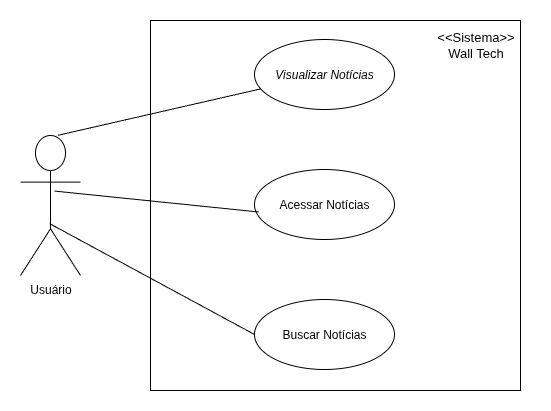
\includegraphics[width=0.7\textwidth]{media/wall_tech_use_case.png}
  \legend{Fonte: os autores.}
  \label{fig:caso-uso-walltech}
\end{figure}



\section{Processo de Desenvolvimento}
\label{section:processo-desenvolvimento}
O processo de desenvolvimento utilizado para construir a plataforma WallTech segue a metodologia ágil \english{Kanban}. Essa metodologia de desenvolvimento ágil é baseada em um quadro de tarefas, no qual cada tarefa é representada por um cartão \cite{gomes2014kanban}. O quadro Kanban é dividido em colunas que representam o estado atual de cada tarefa. As colunas mais comuns são: \english{To Do}, \english{In Progress} e \english{Done}, e o quadro é atualizado conforme as tarefas são realizadas. Além dessas colunas, o processo foi adaptado para incluir colunas adicionais como \english{Docs} e \english{Test}, permitindo que a documentação e os testes fossem gerenciados de forma organizada e eficiente durante o desenvolvimento.

A Figura \ref{fig:kanban-walltech} apresenta um exemplo do quadro Kanban utilizado no \english{GitHub Projects}, mostrando a organização das tarefas e o progresso do desenvolvimento da plataforma WallTech. O quadro reflete a estrutura de colunas adaptada, proporcionando uma visão clara do fluxo de trabalho da equipe, o que facilita o acompanhamento das tarefas em diferentes estágios.

Após a definição das funcionalidades principais do sistema, as tarefas foram inicialmente documentadas como \english{user stories}. As \english{user stories} são descrições simples e compreensíveis das funcionalidades a serem implementadas, permitindo uma comunicação clara entre a equipe de desenvolvimento e as partes interessadas. Cada \english{user story} é associada a um conjunto de requisitos específicos e uma definição de pronto, facilitando a compreensão do que precisa ser desenvolvido.

A partir dessas \english{user stories}, as \english{issues} foram criadas no \english{GitHub Projects}. Cada \english{issue} representa uma tarefa específica que deve ser realizada, baseada nas \english{user stories}. No \english{GitHub Projects}, essas \english{issues} são organizadas nas colunas do quadro Kanban, permitindo que a equipe visualize o progresso de cada tarefa e as mova conforme o andamento do trabalho.

A Figura \ref{fig:kanban-userstories} mostra um exemplo de cartão \english{issue} no \english{GitHub Projects}, ilustrando como as \english{user stories} são transformadas em tarefas e organizadas dentro do quadro Kanban. Cada \english{issue} possui detalhes sobre a tarefa, como descrições, prioridade e prazo, facilitando o gerenciamento e a execução das atividades no time de desenvolvimento.

\begin{figure}[H]
  \centering
  \caption{Exemplo de quadro Kanban no \english{GitHub Projects}}
  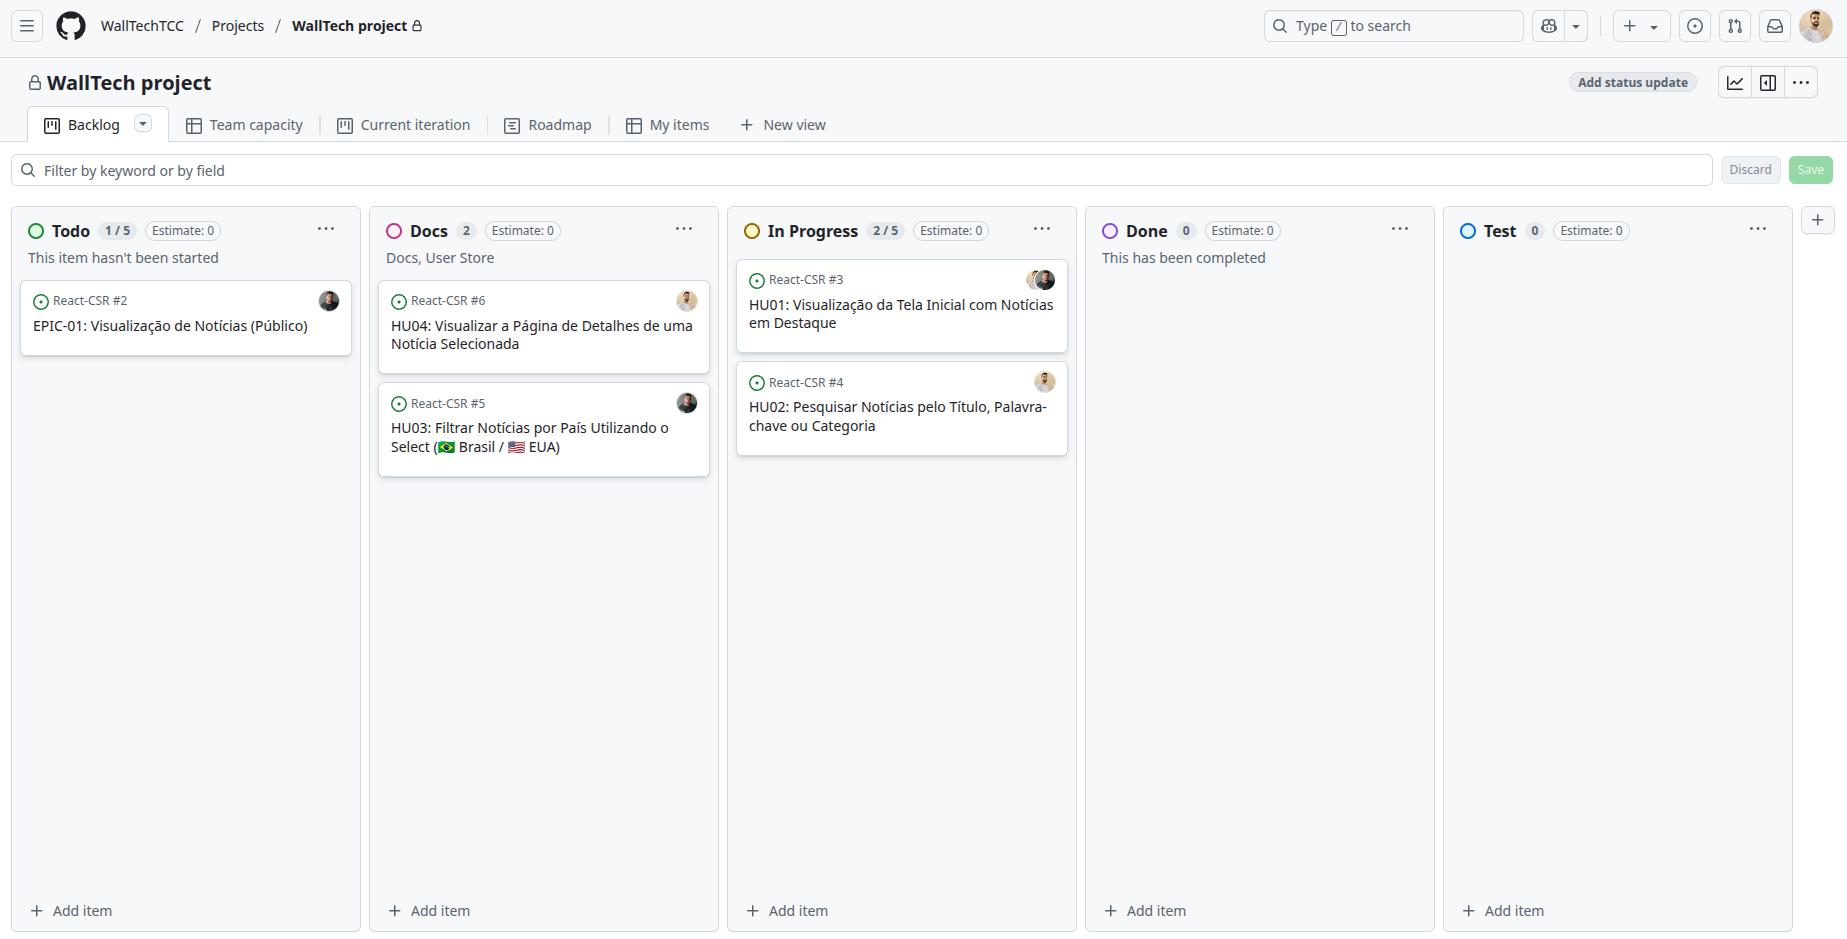
\includegraphics[width=1.0\textwidth]{media/wall_tech_kanban.png}
  \legend{Fonte: os autores.}
  \label{fig:kanban-walltech}
\end{figure}

\begin{figure}[H]
  \centering
  \caption{Exemplo de cartão \english{issue} no \english{GitHub Projects}}
  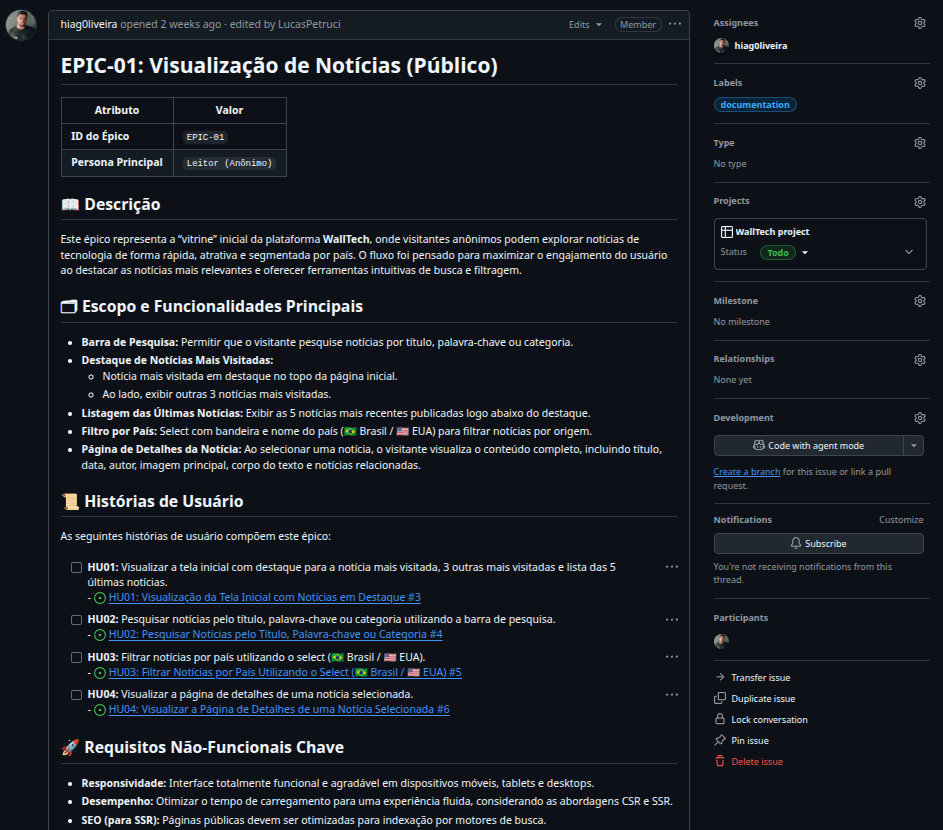
\includegraphics[width=0.7\textwidth]{media/wall_tech_epic.png}
  \legend{Fonte: os autores.}
  \label{fig:kanban-userstories}
\end{figure}

